\documentclass[a4paper,11pt,singlespacing]{article}

\usepackage{setspace}
\usepackage[utf8]{inputenc}
\usepackage[T1]{fontenc}
\usepackage{graphicx}
\usepackage{color}
\usepackage{hyperref}
\usepackage{listings,xcolor}
\usepackage{pdfpages}

\renewcommand{\figurename}{Abbildung}

\graphicspath{ {./images/} }



\begin{document}
	\setlength{\parindent}{0ex}
	
	\begin{titlepage}
		\author{Luca Asmus\\ Marius Würstle\\Rolf Wiersch}
		\title{
\includegraphics[scale=0.3]{rwu_logo_hor-lila-cyan_rgb_0} \\ ~\\ ~\\ WLAN-AP mit regelmäßigem PSK-Tausch und QR-Code Anmeldung \vspace{8cm}}
		\date{\today}
		\maketitle
		\thispagestyle{empty}
    	\end{titlepage}
    	
    	\section{Zusammenfassung}
    	\tableofcontents
    	
    	\section{Abbildungsverzeichnis}
    	\listoffigures
    	\newpage
    	
    	\section{Allgemeines}
    	
    	\section{Fachbegriffe}
    	
    	\section{Hardware}
    		\subsection{Raspberry Pi}
    			Der Raspberry Pi ist wurde für junge Menschen entwickelt, um ihnen eine preisgünstige Möglichkeit zu bieten, sich mit der Informatik zu beschäftigen. Der Einplatinencomputer ist etwa Kreditkartengroß und kam Anfang 2012 auf den Markt. Er ermöglicht einen schnellen und praktischen Weg um Wissen in den Bereichen Programmieren und Hardware. Zudem ist er vielseitig einsetzbar in diesem Fall wird er zu einem Access-Point konfiguriert. 
    			\begin{figure}[ht]
    				\centering
	    			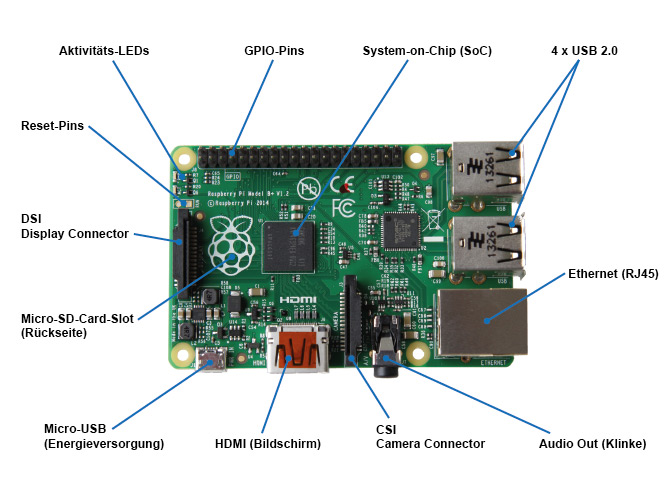
\includegraphics[scale=0.5]{raspberry_pi_3b}
	    				\caption{Raspberry Pi 3b}
	    				\label{raspberrypi3b}
				\end{figure}
				Technische Spezifikationen unseres Raspberry Pi 3b:
				\begin{itemize}
					\item Quad Core 1.2GHz Broadcom BCM2837 64bit CPU
					\item 1GB RAM
					\item BCM43438 wireless LAN and Bluetooth Low Energy (BLE) on board
					\item 100 Base Ethernet
					\item 40-pin extended GPIO
					\item 4 USB 2 ports
					\item 4 Pole stereo output and composite video port
					\item Full size HDMI
					\item CSI camera port for connecting a Raspberry Pi camera
					\item DSI display port for connecting a Raspberry Pi touchscreen display
					\item Micro SD port for loading your operating system and storing data
					\item Upgraded switched Micro USB power source up to 2.5A
				\end{itemize}
			\subsection{Raspberry Pi Shield - Display LCD-Touch, 3,2in}
				Der Touchscreen wertet den Raspberry Pi zu einem vollwertigen Touch-PC auf. Für zusätzliche Funktionen besitzt der Display 3 Buttons an der Seite, welche einfach über die GPIO Pins eingelesen werden können.
				\begin{figure}[ht]
					\centering
					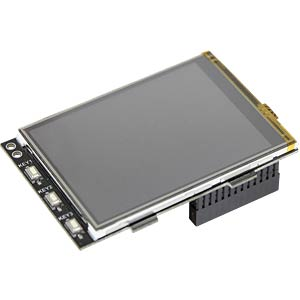
\includegraphics[scale=0.5]{touch_display}
					\caption{Touchscreen Display für den Raspberry Pi}
					\label{touchdisplay}
				\end{figure}
				Technische Spezifikationen unseres Raspberry Pi Shield - Display LCD-Touch, 3.2in:
				\begin{itemize}
					\item Display 8,13cm (3,2")
					\item Auflösung 320 x 240 Pixel
					\item LED-Hintergrundbeleuchtung
					\item 3 frei belegbare Taster (angebunden an GPIO12, 16, 18)
					\item SPI-Schnittstelle
					\item Touchscreen Technologie resistiv
				\end{itemize}
		\subsection{SD-Karte}
    			32GB
    			
    	\section{Software}
    		\subsection{balenaEtcher}
    			Flash Sd Card
		\subsection{hostapd}
    		\subsection{dnsmasq}
    		\subsection{cron}
			Planen der Ausführung des Skripts
    		\subsection{Python3.7}
    			\subsubsection{pyqrcode}
    			\subsubsection{gpiozero}
    	\section{Konfiguration des Raspberry Pi als Access-Point}
    	
    	\section{Passwortgenerierung}
    		Die Passwortgenerierung wird mithilfe eines Python Skripts gelöst. Dieses ist in unserem GitHub repository hinterlegt und für jeden zugänglich (ref zum Link). Das Skript verwendet die zwei Imports string und secrets. Mithilfe der Bibliothek string können die für Bash problematischen Zeichen aus dem Alphabet entfernt werden können. Das secrets Modul wird für das Generieren von stark kryptographischen Passwörter verwendet. Die verwendete Funktion secrets.choice wählt aus der mitgelieferten Sequenz ein Zeichen aus. Welches anschließend an den schon vorhandenen String angehängt. Dies wird 10 mal ausgeführt.
    		\lstset{
    			numbers=left,
    			basicstyle=\ttfamily,
    			language=Python,
    			keywordstyle=\color{blue},
    			commentstyle=\color{green},
    			xleftmargin=1cm
    		}
			\begin{lstlisting}
import secrets
import string

def get_random_password():
temp = string.ascii_letters + string.digits + string.punctuation

alphabet = temp.replace('\'', '').replace('\\', '')
.replace('\"','').replace('\`', '').replace(';', '')

password = ''.join(secrets.choice(alphabet) for i in range(10))
return password

if __name__ == "__main__":
print(get_random_password())
			\end{lstlisting}
    	\section{Ausgabe des Passworts}
    	
    	\section{Fazit mit Ausblick}
    	
    	\section{Quellenverzeichnis}
    	
    	\url{http://www.elektronik-kompendium.de/sites/raspberry-pi/bilder/19052512.jpg} [aufgerufen am 25.11.2020] \ref{raspberrypi3b} \\
    	
    	\url{https://cdn-reichelt.de/bilder/web/artikel_ws/A300/TFTV2.jpg} [aufgerufen am 26.11.2020] \ref{touchdisplay}
\end{document}
